% !TeX encoding = utf8
% !TeX spellcheck = pl_PL

\documentclass[11pt, a4paper, twoside]{article}
\usepackage{graphicx, color, rotating} 
\usepackage[MeX, plmath]{polski} %MeX - tryb pełnej polonizacji
\usepackage[OT4]{fontenc} % T1 - skład fontami EC; OT4 - układ fontów PL
\usepackage{ae,aecompl}
\usepackage[utf8]{inputenc}
\usepackage{lmodern} %czcionka latin modern; jednolita dla tekstu i wzorów;
\usepackage{a4wide}
\usepackage{amsmath}
\usepackage{amssymb, latexsym}
\usepackage{array}
\usepackage{bm}
\usepackage[shortlabels]{enumitem}
\usepackage[font=footnotesize]{caption} %rozmiar czcionki podpisów pod rysunkami
\usepackage{float}
\usepackage{subfig} %obrazki obok siebie
\usepackage[hidelinks]{hyperref}
\usepackage{indentfirst}
\usepackage{geometry}
\geometry{left=25mm, right=25mm, top=25mm, bottom=25mm}

\usepackage[final]{pdfpages}
\usepackage{pdflscape}
\prefixing %notacja prefiksowa w pakiecie 'polski'
\frenchspacing
\linespread{1.1}
\renewcommand{\figurename}{Rys.}
\hyphenation{steer-ing}
%\renewcommand*\thesubsection{\arabic{subsection}} % zmiana numeracji podsekcji 0.X -> X

\begin{document}
	
	\begin{center} 
		{\Large Wydział Elektroniki i Technik Informacyjnych}
		\vskip0.2cm
		{\LARGE \textbf{Sieci i sterowanie systemami (SST): Smart City --~raport końcowy po etapie III projektu } } 
		\vskip0.3cm
		{\Large Szymon Jarocki, Daniel Giełdowski, Maciej Kłos, Michał Okoński}
		\vskip0.8cm
	\end{center} 	
	
Celem ostatniego etapu była ocena skuteczności działania utworzonego oprogramowania. W~związku z~tym przeprowadziliśmy badania eksperymentalne, których wyniki przedstawiamy w~rozdziale~\ref{sec:Wyniki} niniejszego raportu końcowego. Celem uzupełnienia zamieszczamy także podsumowanie projektu i ocenę pracy z~symulatorem.

\label{sec:Wyniki}

%\newpage
\section{Omówienie wyników testów}

Zaprojektowane algorytmy sterowania przetestowano na 3 przykładowych scenariuszach ruchu uszeregowanych pod kątem stopnia trudności.

\subsection{Scenariusz 1 - Wykrywanie kolizji}

W pierwszym scenariuszu zbadano zdolność pojazdów do unikania kolizji. Do wykrywania kolizji pojazdy wykorzystywały czujniki laserowe. Po wykryciu zbliżającej się kolizji, pojazd zatrzymywał się. Po zniknięciu kolizji (np. gdy poprzedzający pojazd ruszył) samochód ruszał ponownie. Przykładowe migawki z symulacji przedstawiono poniżej.

\begin{figure}[!h]
	\centering
	\centering
	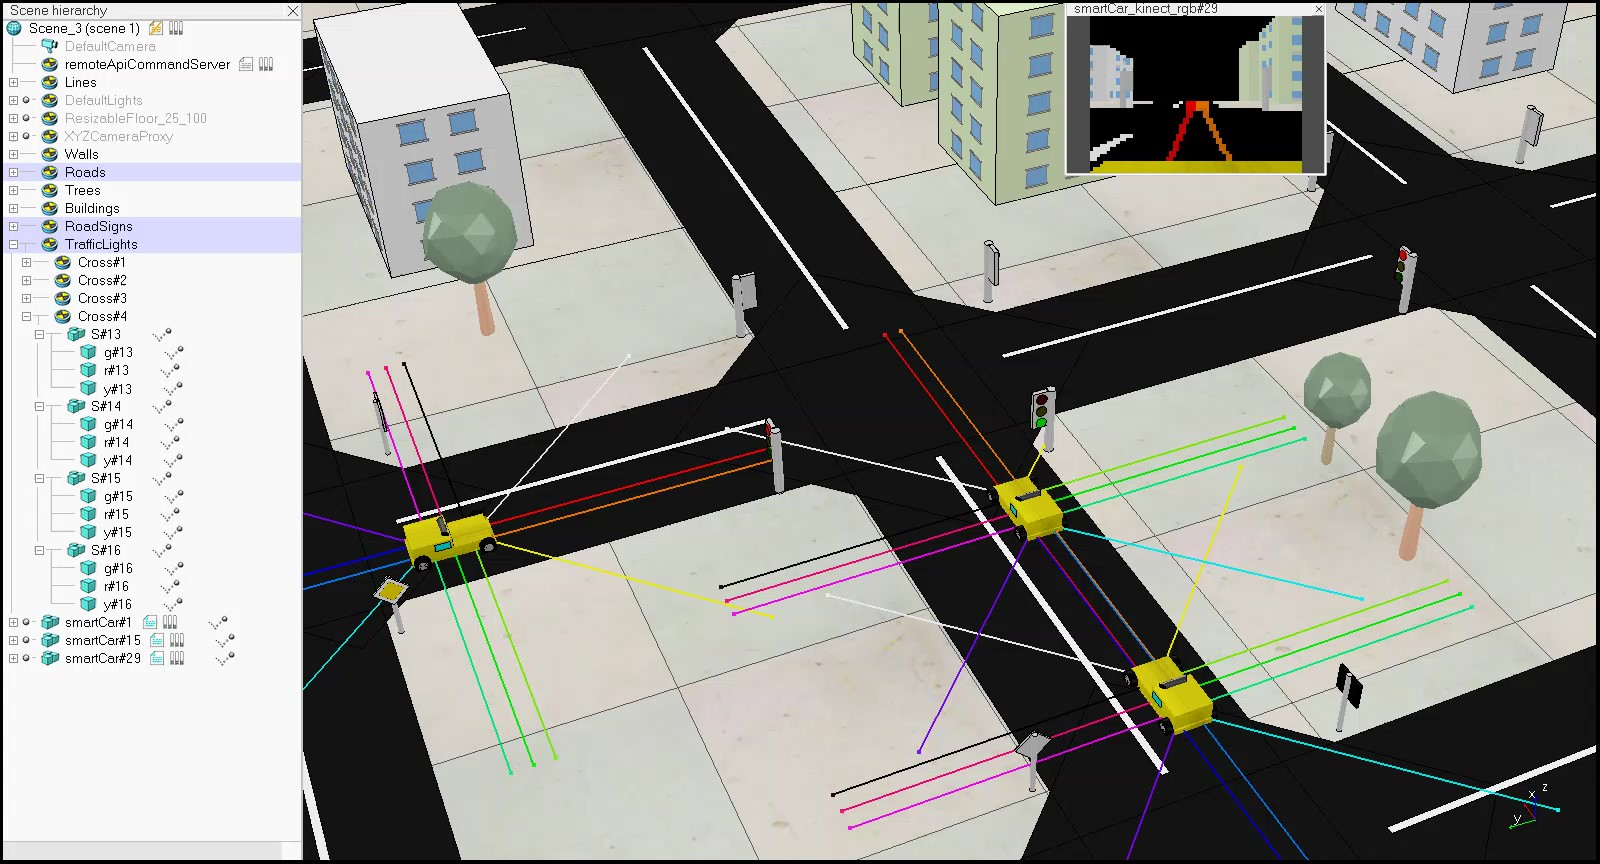
\includegraphics[width=.8\linewidth]{p11.jpg}
	\caption{Początek symulacji - scen. 1}
	\label{fig:p11}
\end{figure}

\begin{figure}[!h]
	\centering
	\centering
	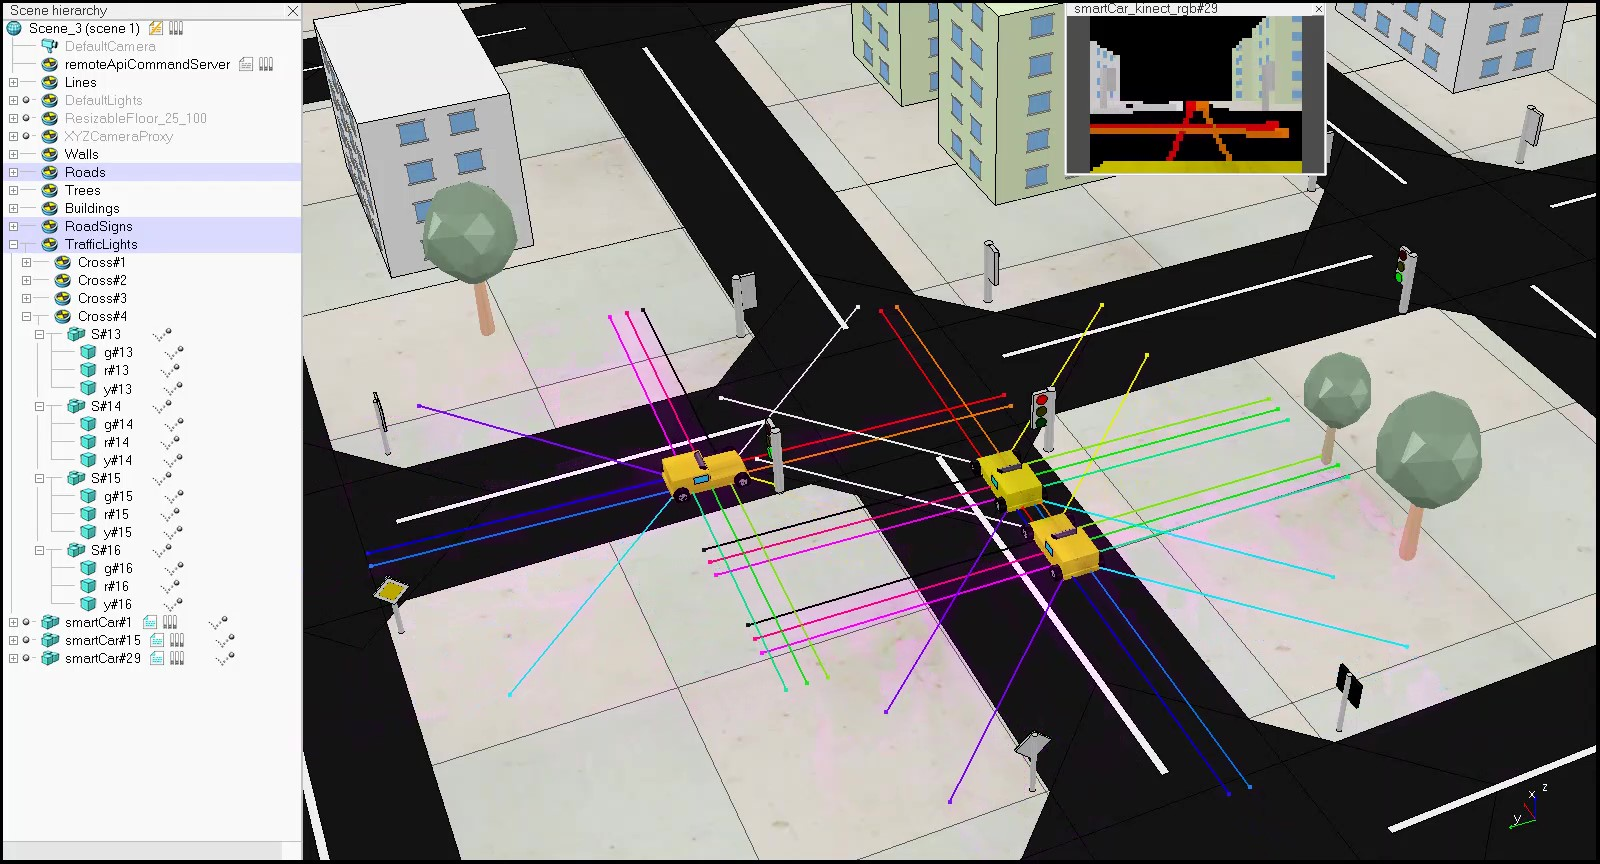
\includegraphics[width=.8\linewidth]{p12.jpg}
	\caption{Wykrycie kolizji po dojeździe do skrzyżowania - scen. 1}
	\label{fig:p12}
\end{figure}

\subsection{Scenariusz 2 - Pokonywanie skrzyżowań}

W drugim scenariuszu zbadano zdolność pojazdów do pokonywania skrzyżowań. Samochody pokonywały skrzyżowania zgodnie z pierwszeństwem wyznaczanym przez zawczasu ustalony priorytet dróg. Samochody zatrzymywały się przed skrzyżowaniem w momencie gdy na drodze o wyższym priorytecie znajdowały się samochody zbliżające się do skrzyżowania. Przykładowe migawki z symulacji przedstawiono poniżej.

\begin{figure}[!h]
	\centering
	\centering
	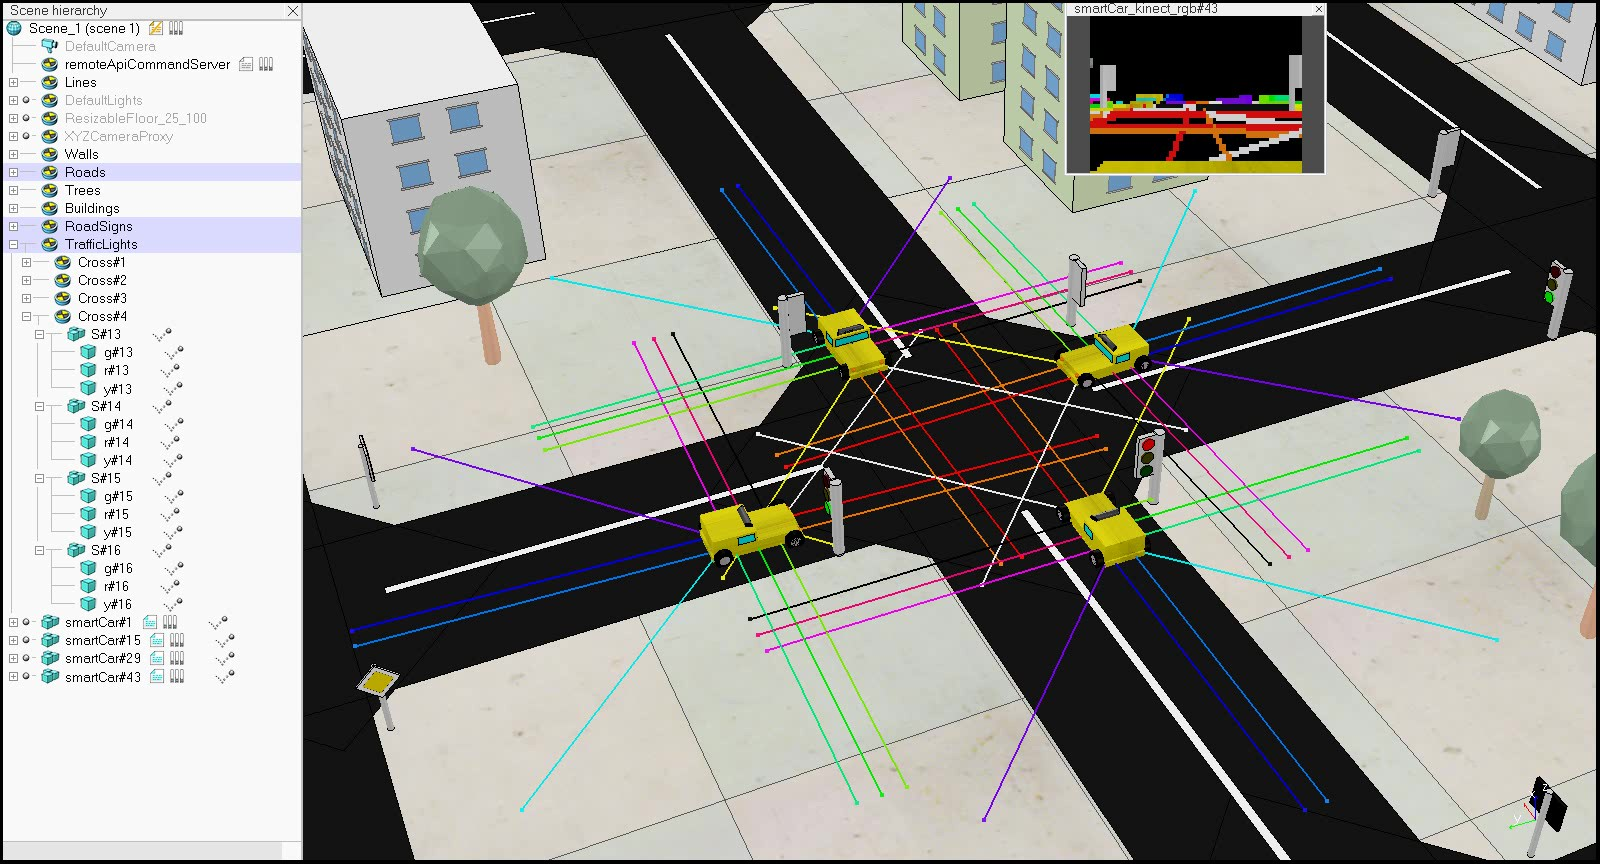
\includegraphics[width=.8\linewidth]{p21.jpg}
	\caption{Początek symulacji - scen. 2}
	\label{fig:p21}
\end{figure}

\begin{figure}[!h]
	\centering
	\centering
	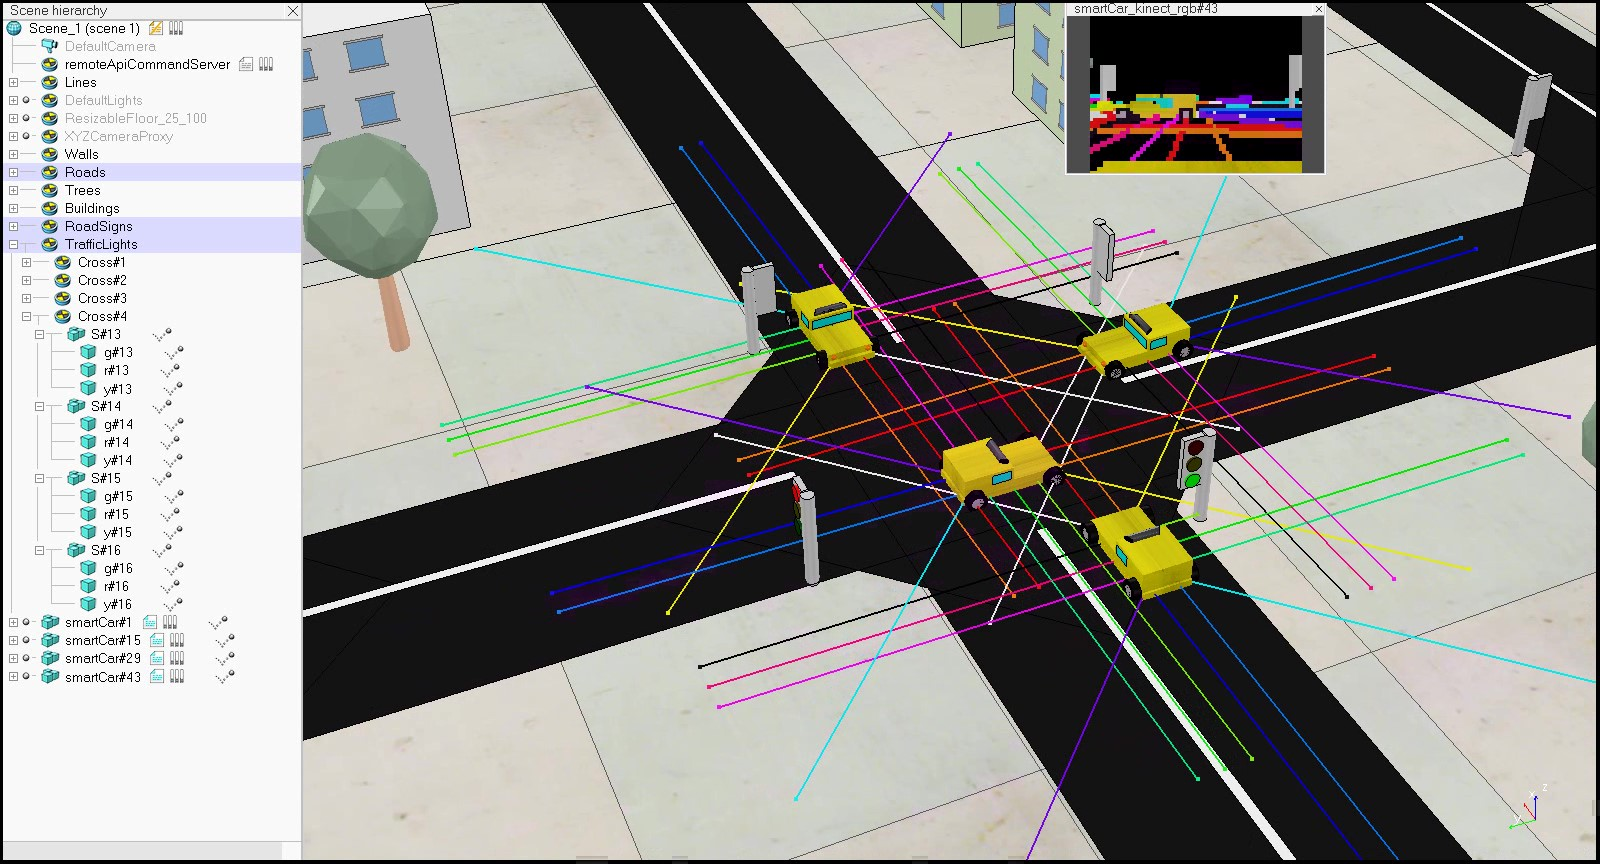
\includegraphics[width=.8\linewidth]{p22.jpg}
	\caption{Przejazd 1. samochodu przez skrzyżowanie - scen. 2}
	\label{fig:p22}
\end{figure}

\begin{figure}[!h]
	\centering
	\centering
	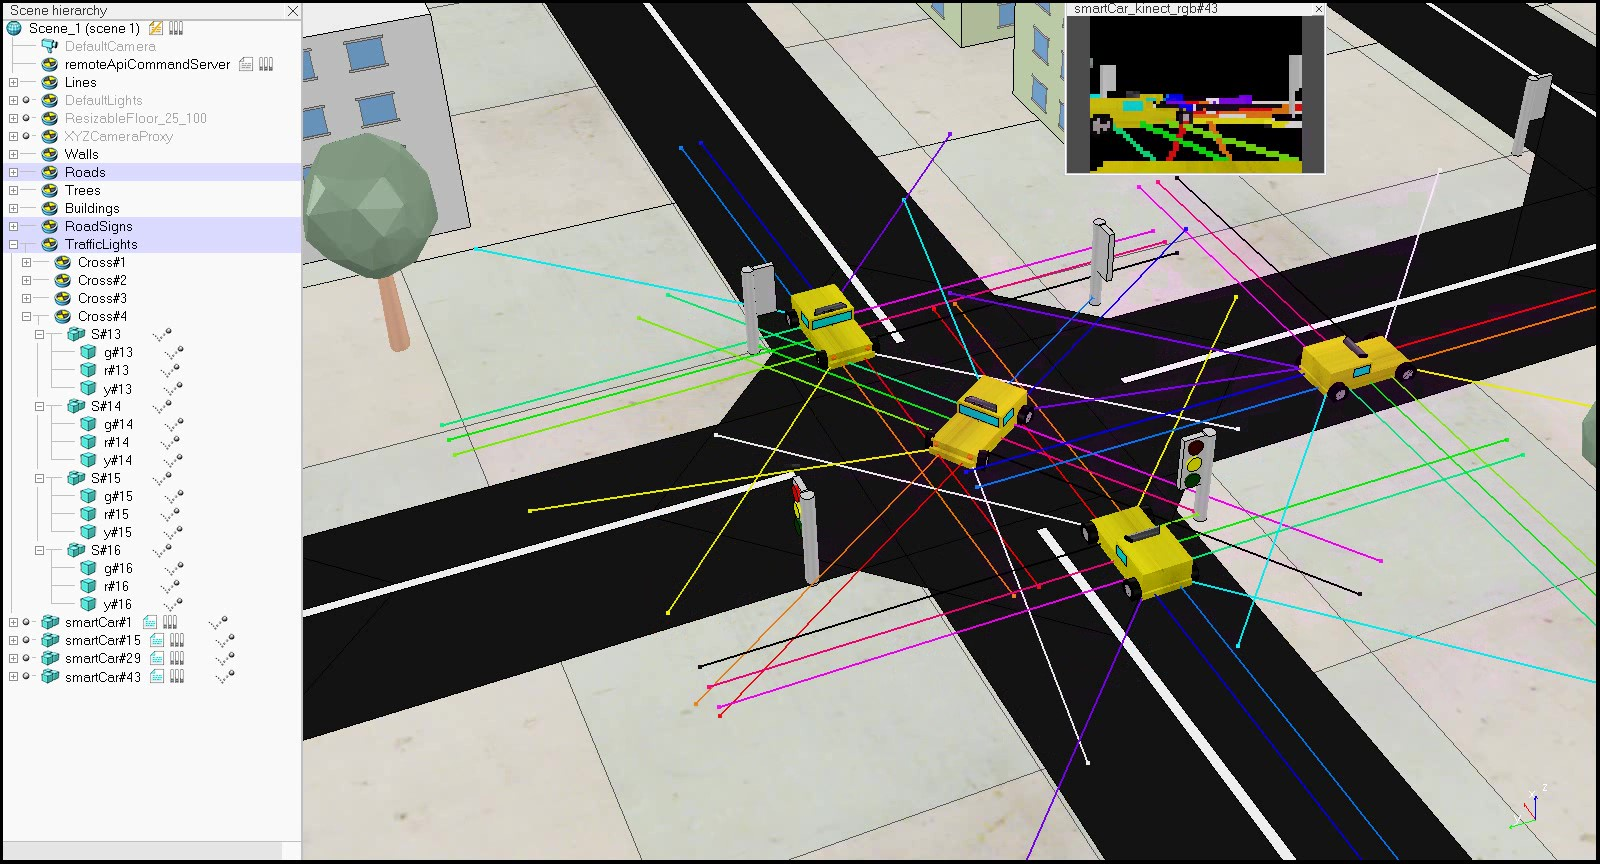
\includegraphics[width=.8\linewidth]{p23.jpg}
	\caption{Skręt w lewo 2. samochodu przez skrzyżowanie - scen. 2}
	\label{fig:p23}
\end{figure}

\begin{figure}[!h]
	\centering
	\centering
	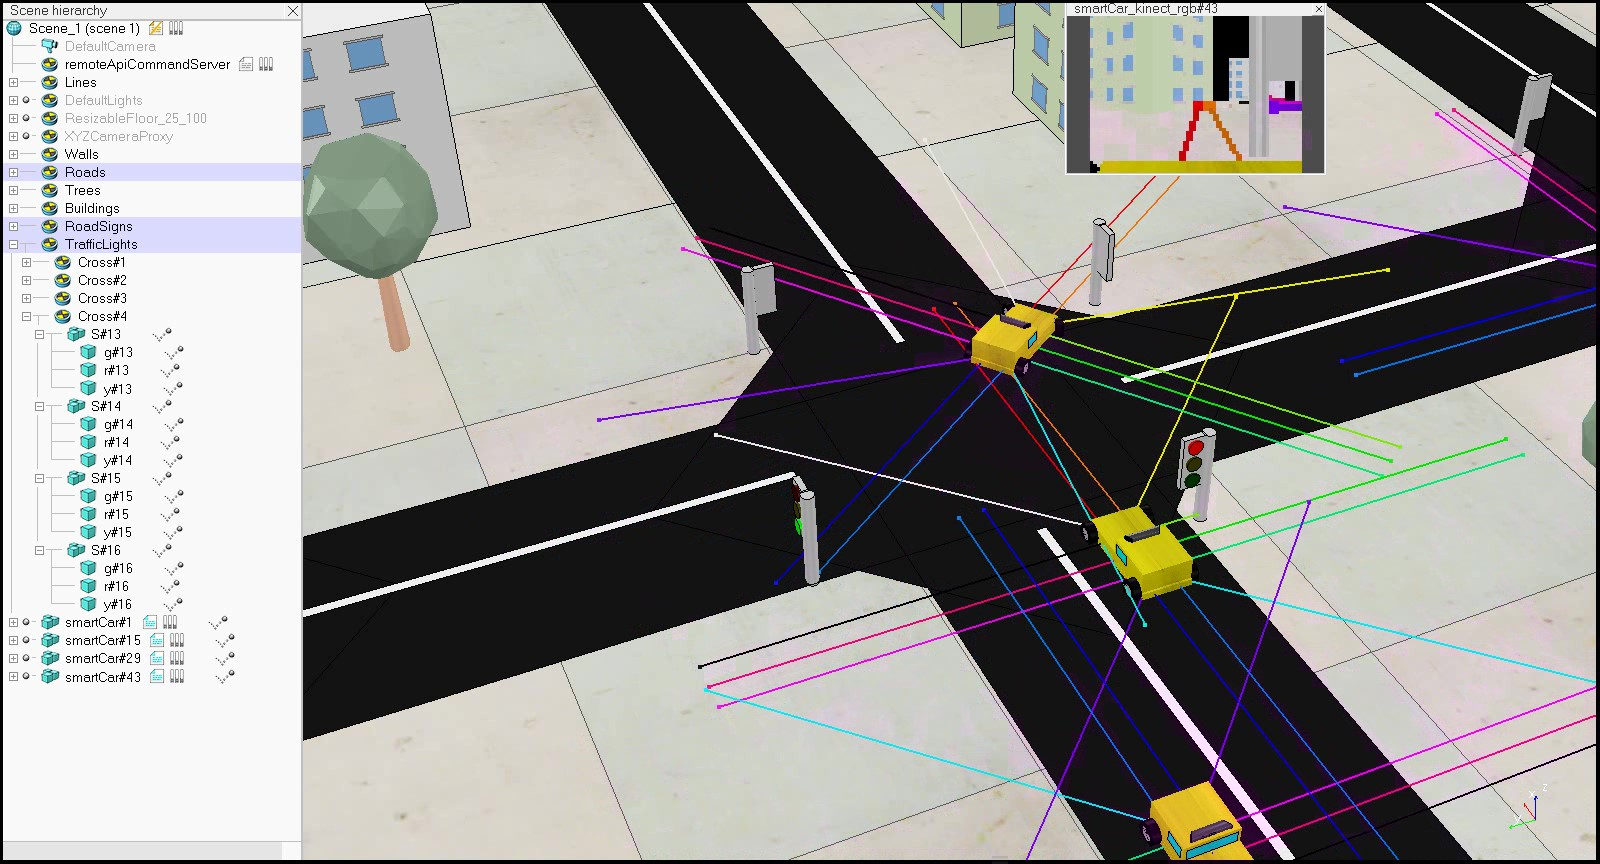
\includegraphics[width=.8\linewidth]{p24.jpg}
	\caption{Zawracanie 3. samochodu na skrzyżowaniu - scen. 2}
	\label{fig:p24}
\end{figure}

\begin{figure}[!h]
	\centering
	\centering
	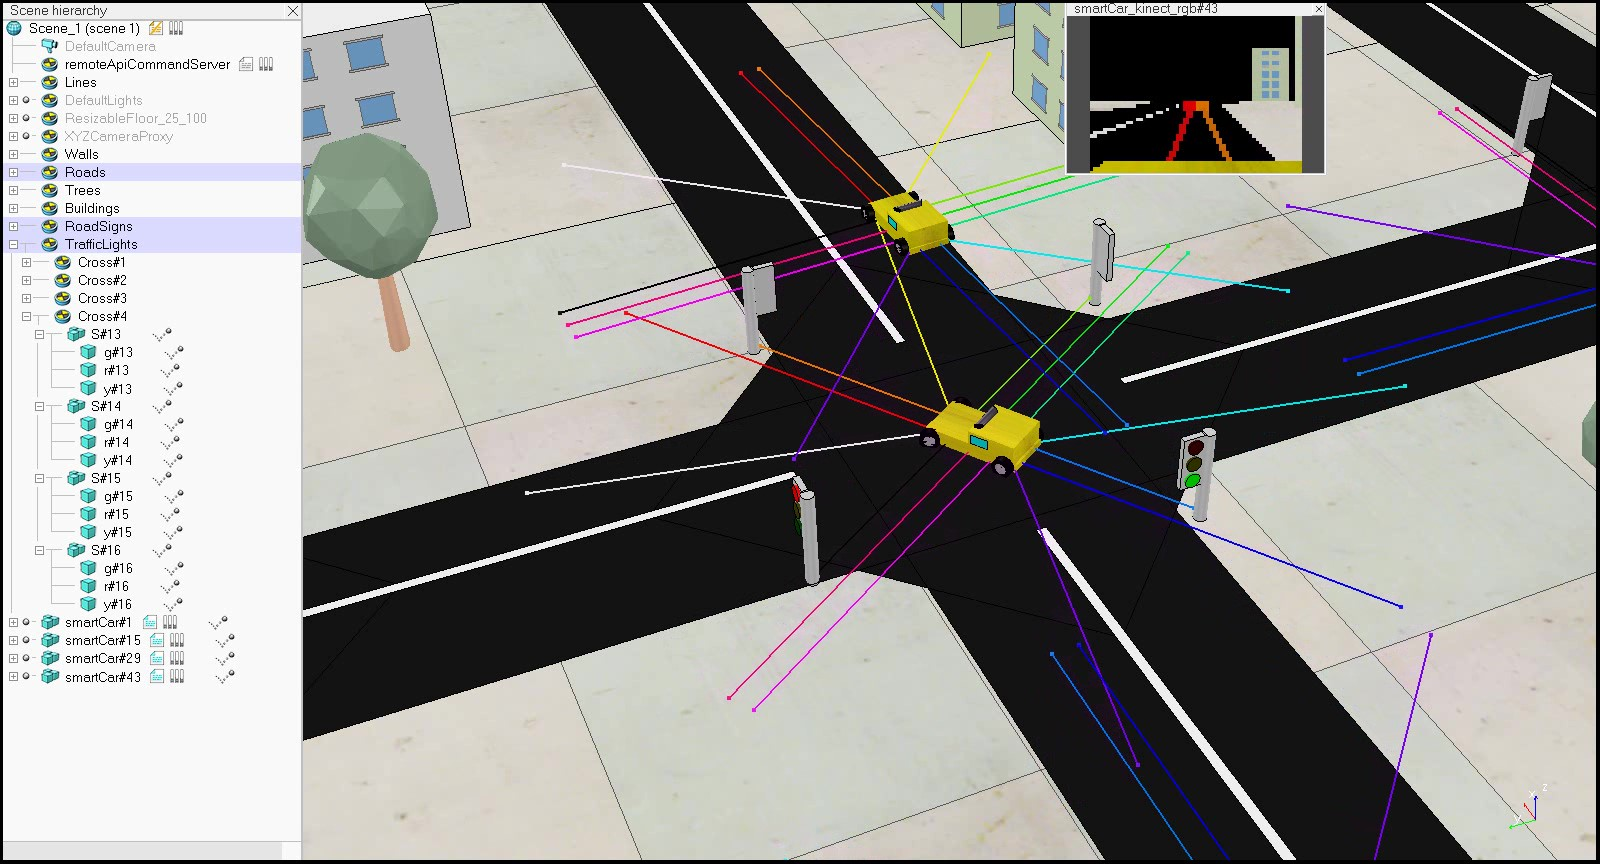
\includegraphics[width=.8\linewidth]{p25.jpg}
	\caption{Zawracanie 4. samochodu na skrzyżowaniu - scen. 2}
	\label{fig:p25}
\end{figure}

\subsection{Scenariusz 3 - Przejazd pojazdów do punktów docelowych}
 
 W ostatnim scenariuszu zbadano zdolność pojazdów do pokonywania zadanych tras w obliczu dużego ruchu. Przeprowadzono symulację z 8 samochodami, którym punkty docelowe zadano w sposób losowy. Przykładowe migawki z symulacji przedstawiono poniżej.
 
 \begin{figure}[!h]
 	\centering
 	\centering
 	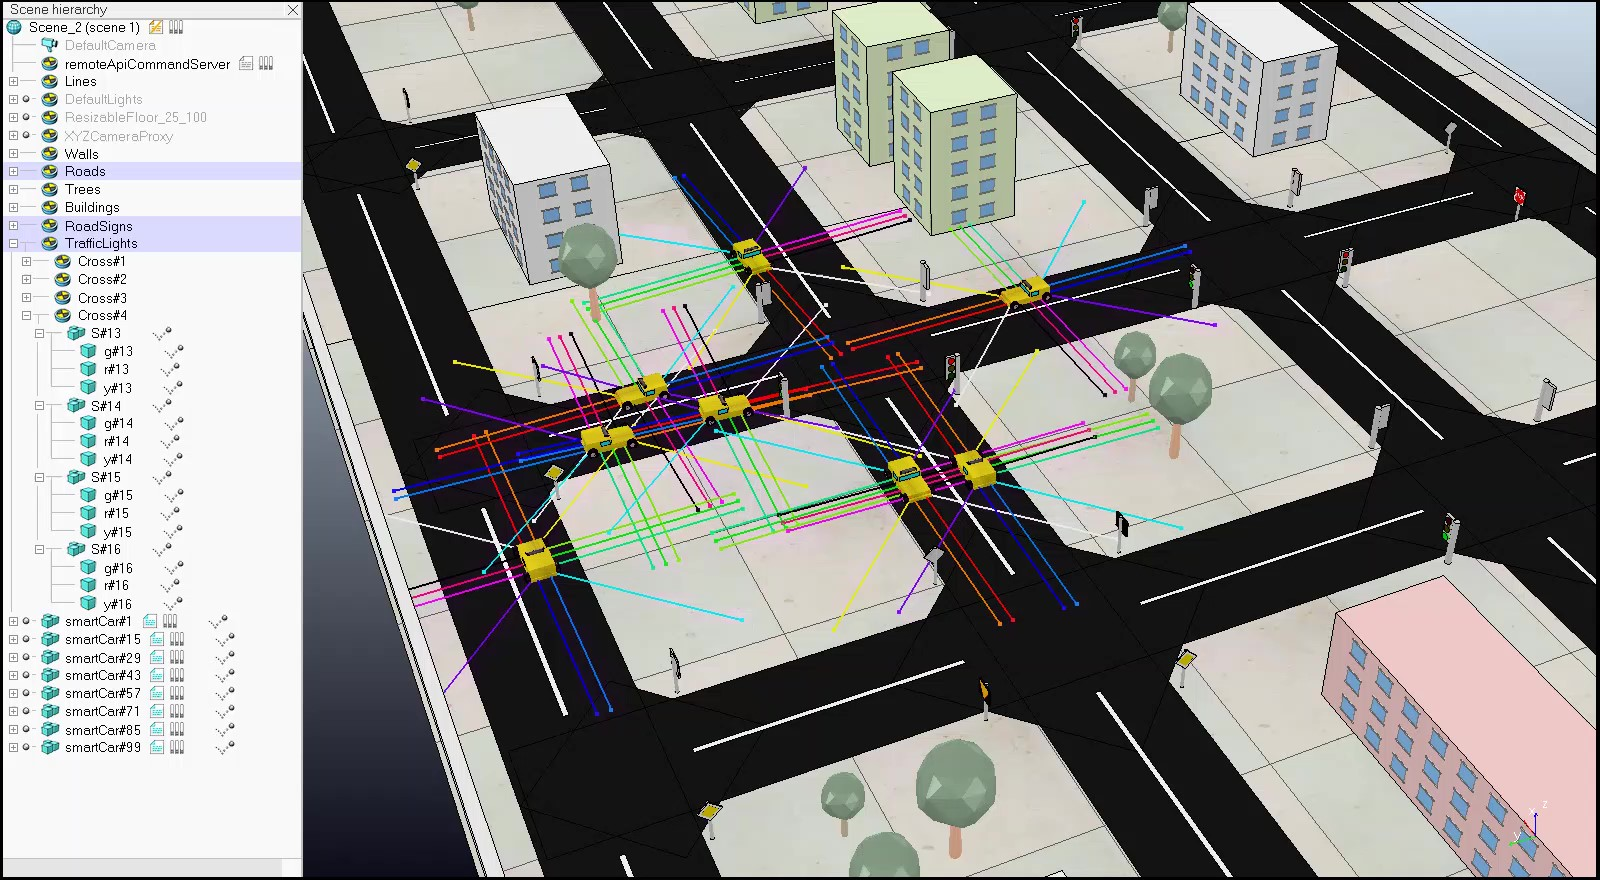
\includegraphics[width=.8\linewidth]{p31.jpg}
 	\caption{Początek symulacji - scen. 3}
 	\label{fig:p31}
 \end{figure}

 \begin{figure}[!h]
	\centering
	\centering
	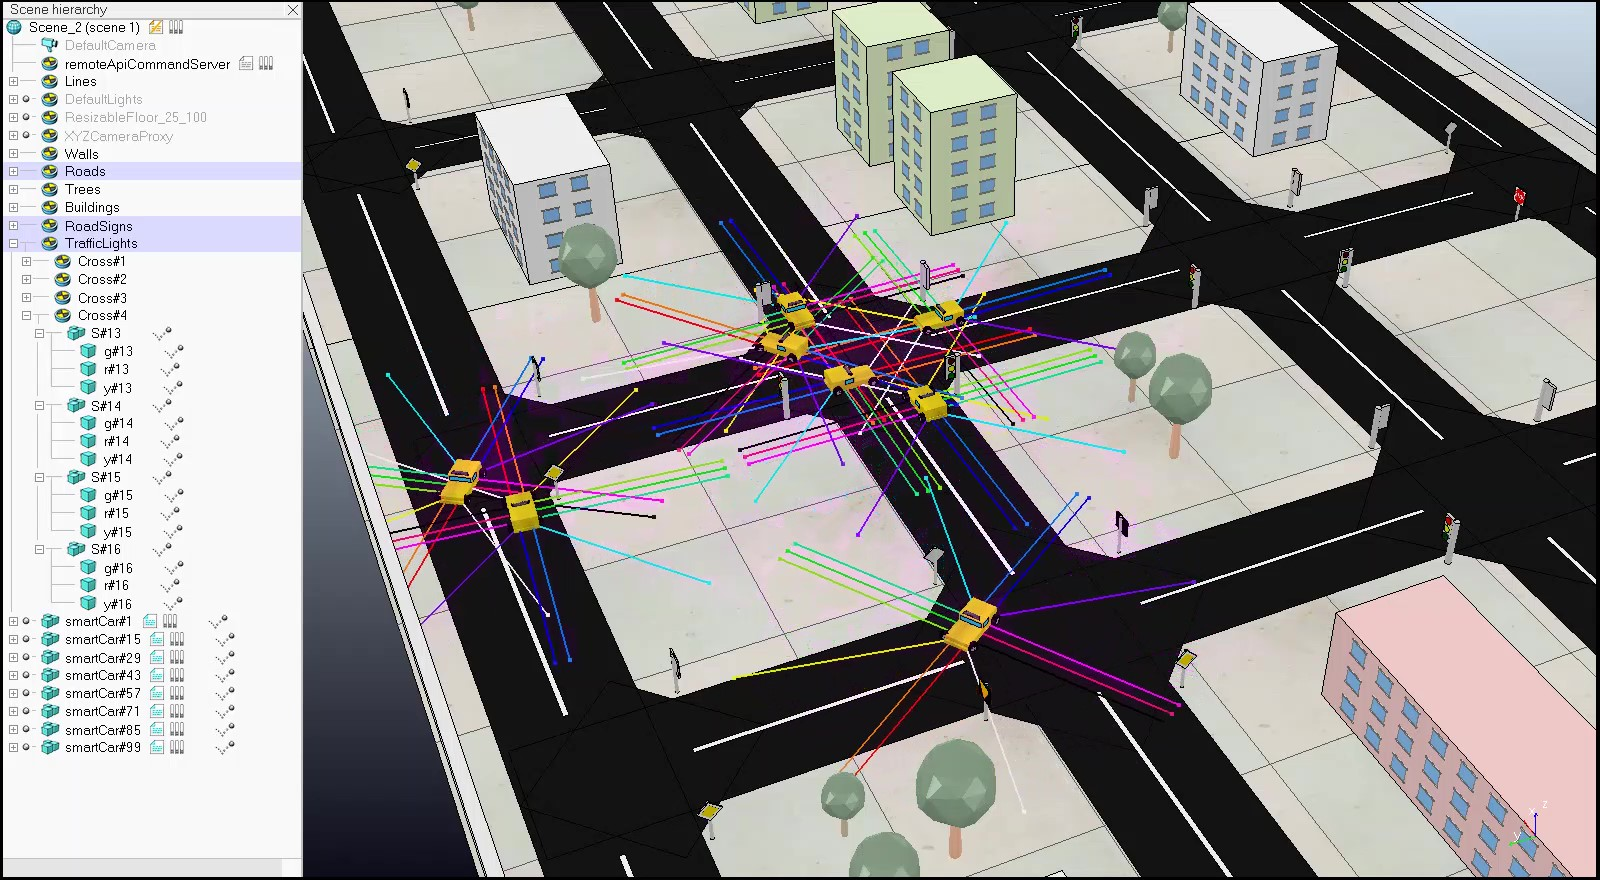
\includegraphics[width=.8\linewidth]{p32.jpg}
	\caption{Migawka z symulacji - scen. 3}
	\label{fig:p32}
\end{figure}

 \begin{figure}[!h]
	\centering
	\centering
	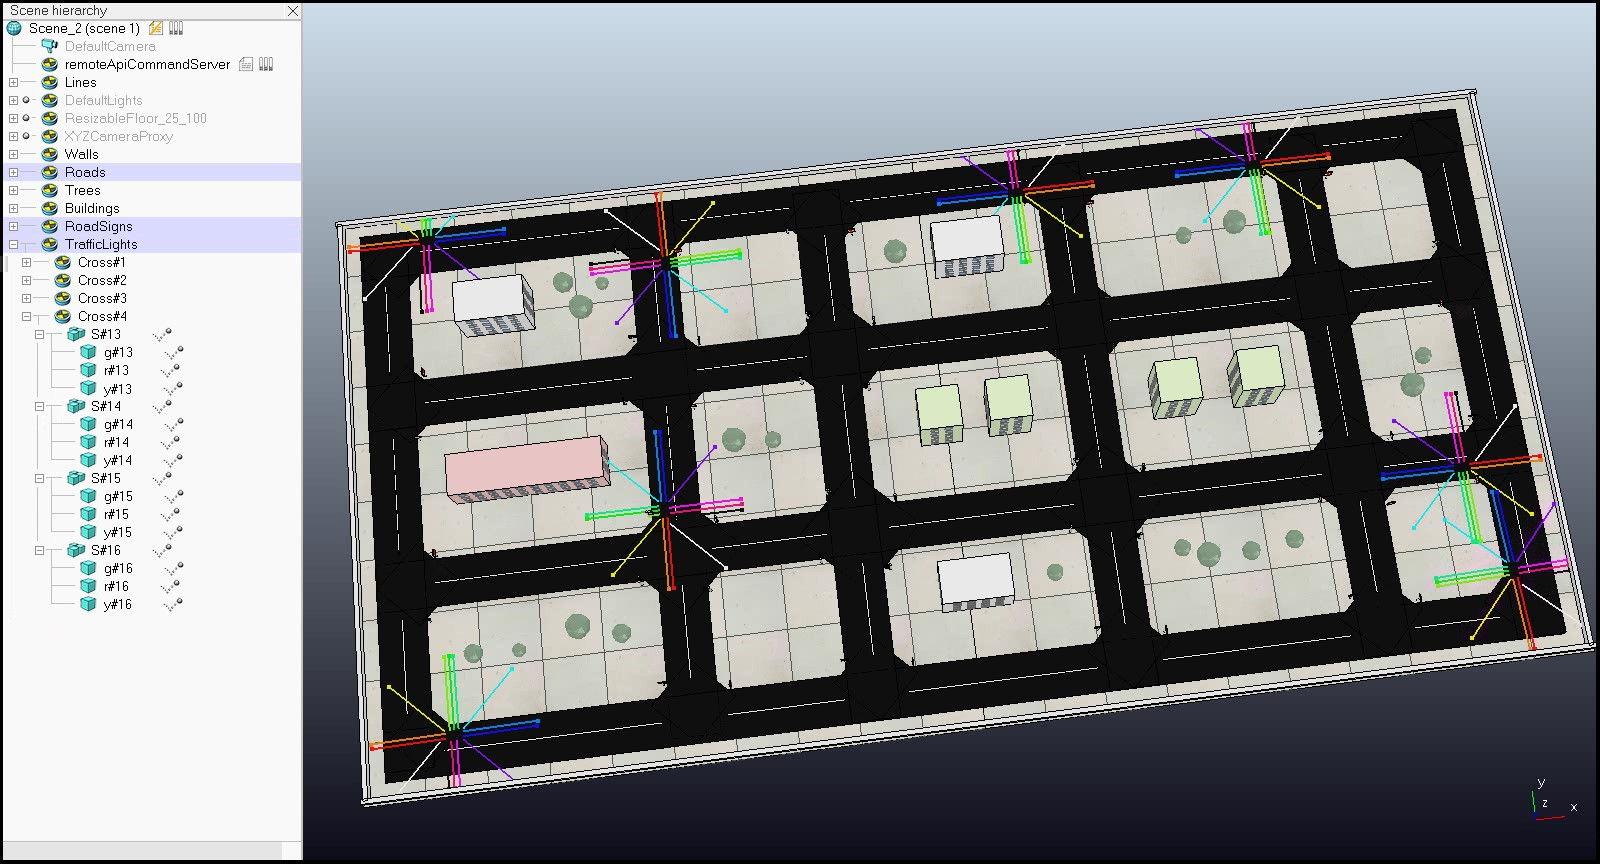
\includegraphics[width=.8\linewidth]{p33.jpg}
	\caption{Koniec symulacji - zaznaczone końcowe pozycje - scen. 3}
	\label{fig:p33}
\end{figure}
 
 
 


\section{Podsumowanie i ocena pracy z symulatorem}
	
	
	
		
\end{document}

